\chapter{Task 4}
\label{chapter:task4}
In this chapter we began to consider irregular array antennas with N identical elements. Array antennas are good to use as they can for example increase the overall gain, provide diversity reception, steer the array in a particular direction and determine the direction of arrival of the incoming signals.\cite{AntennasFundamentals} 

In this section specifically we were considering an array antenna with irregular spacing $\{\mathbf{r}_i\}_{i=1}^N$ and excitation currents $\{I_i\}_{i=1}^N$. A function was created that takes the positions,  and  excitation vector which gave the far field function of the array antenna as output.
 
\section{Theory}
For antennas with identical elements that lie in an arbitrary array the far field function  may be computed as a sum over the elements in the array elements

\begin{equation}
\mathbf{G}_A(\theta, \phi) = \sum_{n=1}^N A_ne^{j\phi_n}(G_{\theta}\hat{\theta} + G_{\phi}\hat{\phi}) e^{jk\mathbf{r}_n\dot{\hat{r}}}.
\end{equation}
Which can be written as 
\begin{equation}
\mathbf{G}_A(\theta, \phi) = \mathbf{G}(\theta, \phi) \cdot AF
\end{equation}
where AF stands for Array Factor. Further $\mathbf{r}_n$ are the positions of the elements (assumed to be given in $m\lambda$), $A_n$ and $\phi_n$ are the amplitude and phase of the current, respectively. The excitation current can be written in terms of amplitude and phase of the current 
\begin{equation}
\mathbf{I} =[A_1e^{j\Phi_1} A_2e^{j\Phi_2} \dots A_{N-1}e^{j\Phi_{N-1}}],
\end{equation}
it is then easy to compute the far field function. \cite{kildal2000foundations} 

\section{Result}
The MATLAB code for this section can be  viewed in appendix \ref{section:task4.m}. The absolute value of the $\theta$ and $\phi$ parts of the  far field function  were plotted in figures \ref{task4:Gth} and \ref{task4:Gphi} with respect to the angles  $\theta$ and $\phi$, respectively. 

\begin{figure}[h]
\centering
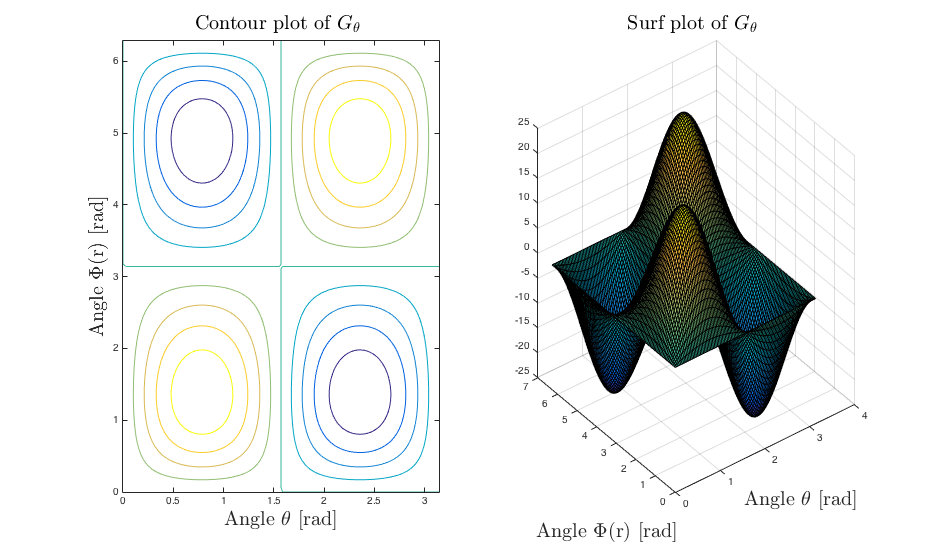
\includegraphics[scale=0.4]{/Users/marikasvensson/Documents/MATLAB/MicroProject/finished/task4/Gth.png}
\caption{This figure shows $G_\theta$ as a function of $\theta$ and $\phi$}
\label{task4:Gth}
\end{figure}


\begin{figure}[h]
\centering
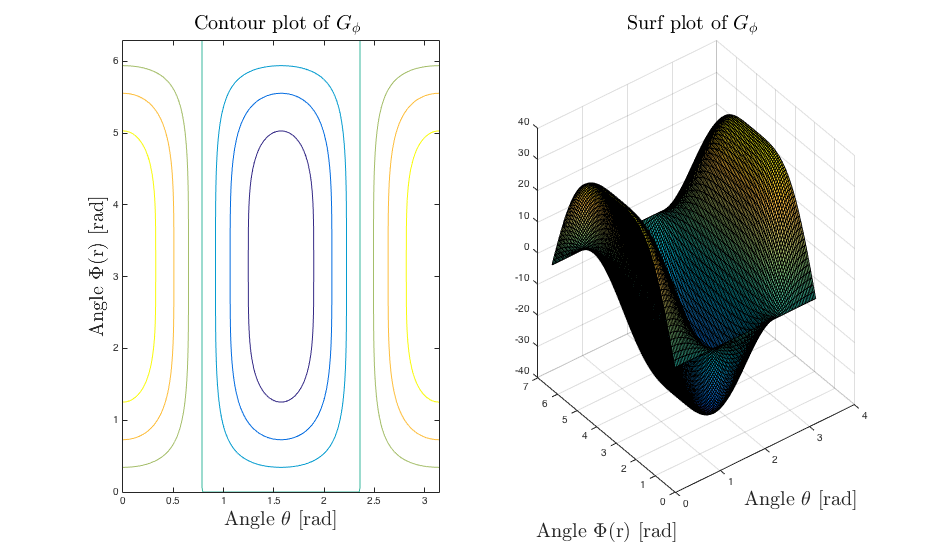
\includegraphics[scale=0.4]{/Users/marikasvensson/Documents/MATLAB/MicroProject/finished/task4/Gphi.png}
\caption{This figure shows $G_\phi$ as a function of $\theta$ and $\phi$}
\label{task4:Gphi}
\end{figure}

